%\documentclass[aps,prl, reprint]{revtex4-1}
\documentclass[11pt,oneside,a4paper, captions=nooneline, headsepline]{article}%was
\usepackage{graphicx}% Include figure files
\usepackage{dcolumn}% Align table columns on decimal point
\usepackage{bm}% bold math
\usepackage[english]{babel}
\usepackage[utf8]{inputenc}%macht ö sichtbar
\usepackage{graphicx}
%\usepackage{natbib}
\usepackage[numbers,square]{natbib}
\bibliographystyle{plain}
%\bibliographystyle{aipauth4-1}
\usepackage{amsfonts}
\usepackage{amsmath}
\usepackage{cancel}
\usepackage{graphicx}
\usepackage{mathcomp}
\linespread{1.3} % 1,5facher Zeilenabstand
\marginparwidth = 25pt
\oddsidemargin = 21pt
\textwidth = 420pt
\hoffset= 0pt
\title{\huge{Construction of an EMT-PES for a Hydrogen Atom at a Metal(111) Surface}}
\begin{document}
\maketitle
\section*{Overview}
The procedure to procure a H@Metal(111)-GGA-PES with VASP is to do 1) Bulk-calculations: calculate the lattice constant for the chosen functional, 2) Slab-calculations: calculate the interlayer distance to obtain a fully relaxed slab, 3) Optimise the H@Metal-system, 4) Map out an energy grid, and 5) Fit to Effective Medium Theory.\\
1) to 6) involve VASP-calculations. The POTCAR-file stays the same for 1) and 2) and is joined with the POTCAR-file for H for 3) and 4). The other input-files needed are the POSCAR-file, which contains the position of the atoms; the INCAR-file, which contains options for VASP; and the KPOINTS-file which determines the sampling of the brillouin-zone.\\
\textbf{All files, most of all the INCAR-file, should be kept minimal to minimise mistakes.}\\
Information summed up here for the VASP-calculation is usually taken from the VASP-manual (http://cms.mpi.univie.ac.at/vasp/vasp/vasp.html, as of 15.01.15, 10:30.).

\section{Bulk-Calculations}
\label{bulk}
Purpose:\\
The Bulk-calculations determine the lattice constant corresponding to the chosen GGA-functional, because GGA-functional do not reproduce the experimental lattice constant but have their own, internal lattice constant.\\
Optimisation:\\
Optimisation needs to be done to get the best result with the lowest computational effort. For that, several input parameters for VASP should be checked:\\
\textbf{ENCUT}: The cut-off. The smaller this radius, the lower the computational effort. If it is too small, though, necessary contributions are neglected. Vary in steps of 50 eV.\\
\textbf{K-points}: The k-points are the mesh with which the brillouin-zone is sampled in reciprocal space. The larger the number of k-points, the more accurate the sampling. But a large number of k-points also increases the computational effort. Do calculations with 8 to $\sim$35 k-points\\
\textbf{ISMEAR}: This parameter determines the smearing. For bulk and slab do ISMEAR=$1$ for Methfessel-Paxton. You can also check other forms of smearing, but you do not need to.\\
\textbf{SIGMA}: This parameter is related to the entropy in the system. It needs to be checked and adjusted at the end of the calculations. For the beginning, set SIGMA = 0.2. After the lattice constant is determined, vary SIGMA between 0.01 and 0.5 and check the entropy as explained below. The entropy should be less than 1\,meV. Too large smearing values SIGMA might lead to a wrong energy, but too low values require a larger kpoint-mesh. It should be as large as possible in order to minimise the difference between the free energy and the total energy.\\
\textbf{IBRION}: The algorithm with which the ionic positions are updated and moved. $1$ and $2$ are both reasonable choices and should give the same result.\\
\subsubsection*{The POSCAR-file}
\begin{figure}[h!]
\begin{verbatim}
 fcc Au
  a0
  0.5 0.5 0.0
  0.0 0.5 0.5
  0.5 0.0 0.5
    1
 cartesian
 0 0 0
\end{verbatim}
\caption{An exemplary POSCAR-file for the Bulk-Calculations. "a0" indicates where the lattice constant needs to be placed.}
\label{bposcar}
\end{figure}
The POSCAR-file (cf Fig.\,\ref{bposcar}) has the following structure: The first line is a comment-line. In the second line (Fig.\,\ref{bposcar}), the lattice constant $a_0$ is given. Then, from line 3 to 5, the cell matrix needs to be specified. In line 6, the number of atoms per cell is given, followed in line 7 by the coordinate system in which the coordinates of the atoms are given from line 8 downwards. Due to the periodic boundary conditions onyl one atom per sell is needed for the bulk calculations. This results in a $1\times1\times1$ cell.
\subsubsection*{KPOINTS-file}
\begin{figure}[h!]
\begin{verbatim}
K-Points
 0
Gammacentered
 8 8 8
 0  0  0
\end{verbatim}
\caption{An exemplary KPOINTS-file for the Bulk-Calculations.}
\label{bkp}
\end{figure}
The structure for the KPOINTS-file is as follows (cf Fig.\,\ref{bkp}): The first line is a comment-line, followed by the number of k-points. If that number is set to zero, the k-point mesh is set automatically. It is best to leave it at that. The third line expresses where the mesh should be centred (in the example on the Gamma-point of the Brillouin zone), the number of k-points for each coordinate $x$, $y$ and $z$ are given in line four and in the last line, the shift of the kpoints can but need not be expressed.\\
\subsection{General Procedure}
To calculate the lattice constant, one starts with initial guesses for the lattice constant in the POSCAR-file (Fig.\,\ref{bposcar}, ``$a_0$"). Example: The experimental lattice constant for Au is $a_0=4.08$\,\AA. To get the GGA-lattice constant, $a_0$ is varied from $3.8$ to $4.4$\,\AA~in steps of 0.1\,\AA.\\
The lattice constant can be calculated in two different ways which differ in the input of the INCAR-file. The KPOINTS- (Fig.\,\ref{bkp}) and POSCAR-file (Fig.\,\ref{bposcar}) are the same for both options.


\subsubsection*{Lattice Constant by changing the cell volume}
VASP gives the option to relax the cell volume (ISIF = 7 in the INCAR-file, Fig.\,\ref{bincar1}). That means that for each POSCAR with their different lattice constants, VASP will try to minimise the stress imposed by the imposed lattice constant $a_0$ and end up with new cell-vectors after the calculation that represent a less strained cell.
\begin{figure}[h!]
\begin{verbatim}
System=Bulk Au
ISTART=0		! WAVECAR isn't read in
ICHARG=2		! CHGCAR or CHG aren't read in

PREC=Accurate
EDIFF=1E-05		! 1st accuracy parameter
EDIFFG=-1.0E-03	! 2nd accuracy paramter

ISMEAR=1		! smearing
SIGMA=0.2		! entropy-related
ALFO=Fast

NSW=100			!number of ionic steps during relaxation
ISIF=7
IBRION=2
POTIM=0.6

GGA=RP		! RPBE-GGA-functional
\end{verbatim}
\caption{An exemplary INCAR-file for calculation of lattice constant via cell volume}
\label{bincar1}
\end{figure}
To evaluate the result, look at the end of the OUTCAR-file for the line "VOLUME and BASIS-vectors are now :" and read the new cell-matrix printed below the line `direct lattice vectors' (cf Fig.\,\ref{boutcar1}).\\
In the POSCAR-file used above, you can see that the components of the cell-matrix are either calculated by multiplying the lattice constant by 0.5 or 0.0. To get the new lattice constant, you can now, for example, take the first element of the first lattice vector. Since it is given as 0.5 in your input-POSCAR-file, to calculate the new lattice constant, you now need to multiply the value from the OUTCAR-file by 2. Example (Fig.\,\ref{boutcar1}): The first element of the cell matrix in the OUTCAR-file is $2.055159357$\,\AA. In the POSCAR-file (Fig.\,\ref{bposcar}), the first element of the first lattice vector is $0.5$. To get the new lattice constant, you need to calculate $2.055159357/0.5=4.110$\,\AA. Your new lattice constant is therefore $a_0=4.110$\,\AA.
\begin{figure}[h!!]
\begin{verbatim}
 VOLUME and BASIS-vectors are now :
 -----------------------------------------------------------------------------
  energy-cutoff  :      229.94
  volume of cell :       17.36
      direct lattice vectors                 reciprocal lattice vectors
     2.055159357  2.055159357  0.000000000     0.243290136  0.243290136 -0.243290136
     0.000000000  2.055159357  2.055159357    -0.243290136  0.243290136  0.243290136
     2.055159357  0.000000000  2.055159357     0.243290136 -0.243290136  0.243290136

  length of vectors
     2.906434236  2.906434236  2.906434236     0.421390877  0.421390877  0.421390877

\end{verbatim}
\caption{An exemplary OUTCAR-file for calculation of lattice constant via cell volume}
\label{boutcar1}
\end{figure}
But, if the initial guess is bad, VASP cannot relax the cell enough to get the perfect lattice constant. Therefore, it is necessary to try out several guesses and choose that lattice constant which is closest to its initial guess. It will also be the lattice constant to which most of the other initial guesses converge to.\\
\subsubsection*{Lattice Constant by energy}
With the INCAR-option ISIF=2 (cf Fig.\,\ref{bincar2}), VASP relaxes the ionic positions. Please remember that you always need to specify IBRION = 1 or 2 if you want to activate ISIF. To evaluate the result, look at the end of the OUTCAR-file for the line `` energy(sigma$\rightarrow$0) = " and read in the energy. The initial guess with the lowest energy will be very close to the correct lattice-constant. If you fit a parabola through your inital-guess/energy-points, the minimum of the parabola will give the lattice constant.\\
\begin{figure}[h!!]
\begin{verbatim}
SYSTEM = Au: fcc
ENCUT = 300     
PREC = Normal   
LREAL = .False. 
SIGMA = 0.2
ISMEAR = 1              
GGA = 91       

NSW = 150      
IBRION = 1
ISIF =2     
POTIM = 0.5     
\end{verbatim}
\caption{An exemplary INCAR-file for calculation of lattice constant via energy}
\label{bincar2}
\end{figure}

After the calculations for different ENCUTs and k-points (and which ever parameter was varied) are finished, the true lattice constant and the best set of parameters is chosen in the following manner:\\
Plot the lattice constant for different k-points. For large k-points, the lattice constant should converge to a certain value. This value should be regarded as the optimal value. Now, to get the best k-point set for further calculation, choose the lowest number of k-points that roughly (that is, within 0.001 eV or lower) reproduces your lattice constant. For the other VASP-parameters you varied proceed accordingly.\\
Lastly, the SIGMA-parameter needs to be checked.\\
For that, vary the parameter SIGMA between 0.01 and 0.5. Once the calculations are done the entropy needs to be determined. This can be done in two different way. You can check in the OUTCAR-file for the lowest occurrence of the line ``entropy T*S    EENTRO =" (cf. Fig.\,\ref{ent1}), or you can calculate the difference between the free energy and the energy without entropy. Both should be less tan 1\,meV. SIGMA should be as large as possible without compromising the energy of the system, so choose the largest SIGMA whose energy still corresponds to the energy of the calculations with lower SIGMA.\\
\begin{figure}[h!!]
\begin{verbatim}
 Free energy of the ion-electron system (eV)
  ---------------------------------------------------
  alpha Z        PSCENC =       116.98128788
  Ewald energy   TEWEN  =      -950.74055391
  -1/2 Hartree   DENC   =      -103.57651771
  -V(xc)+E(xc)   XCENC  =      -424.26980779
  PAW double counting   =          .00000000         .00000000
  entropy T*S    EENTRO =         -.00002139
  eigenvalues    EBANDS =         -.66210617
  atomic energy  EATOM  =      1360.63085531
  ---------------------------------------------------
  free energy    TOTEN  =        -1.63686377 eV

  energy without entropy =       -1.63684238  energy(sigma->0) =       -1.63685664  
\end{verbatim}
\caption{Finding the entropy in the OUTCAR-file.}
\label{ent1}
\end{figure}
\section{Slab-Calculations}
\label{slab}
Purpose:\\
The metals-slab terminates at the end of the surface to the vacuum. For the atoms of at least the surface layer neighbours are missing. This can lead to a contraction or expansion of the interlayer distance of the first few layers of the slab. In theory, it can also lead to a reconstruction of the surface's geometry (cf e.g. herringbone reconstruction of Au(111)). Since the reconstruction usually takes place in larger unit cells than we can consider here, we omit reconstruction in $x$ and $y$-direction and only consider the interlayer-relaxation in $z$-direction.\\
For this, we fix the $x$ and $y$-coordinates of all atoms in the system and let the $z$-coordinate relax for all layers but the lowest two layers. The $z$-coordinates of the lowest two layers need to be fixed, too, to prevent the slab from drifting through space in $z$-direction and to give the above layers the impression that they are sitting on a metal-bulk.
\subsection{KPOINTS}
In the KPOINTS-file, a surface needs to be considered now by setting the last k-point to 1 (Fig.\,\ref{slabkp}).
\begin{figure}[h!!]
\begin{verbatim}
K-Points
0
Gammacentered
17 17 1
0 0 0
\end{verbatim}
\caption{Exemplary KPOINTS-file for the slab-relaxation.}
\label{slabkp}
\end{figure}
\subsection{POSCAR}
\begin{figure}[h!!]
\begin{verbatim}
  Au(111)  1 x 1  vac= 13.0000000000000000  A nlayer=  4
  1.000000
   2.970555537    .000000000    .000000000
  -1.485277768   2.572576696    .000000000
    .000000000    .000000000  20.276200000
   4
Selective dynamics
Cartesian
   .000000000   .000000000   .000000000  F  F  T
  1.485277813   .857525591 -2.425400000  F  F  T
   .000000000  1.715051182 -4.850800000  F  F  F
   .000000000   .000000000 -7.276200000  F  F  F
\end{verbatim}
\caption{Exemplary POSCAR-file for the slab-relaxation. Please note that the lattice constant has been multiplied into the cell-matrix and the coordinates and is therefore set to 1.0 in line 2.}
\label{spos}
\end{figure}
In the POSCAR-file, we now need to construct a slab. The first step for this is forcing the periodic boundary conditions to see a slab of metal and not a bulk as before. We do that by enlarging the cell in $z$-direction and leaving part of the space without any atoms, that is, we create a vacuum of a certain thickness $vac$ above our slab. Because the periodic boundary conditions consequently do not replicate our single atom from the bulk-calculations in $z$-direction to form a continuous bulk, there is only one single layer of metal if only one atom is placed in the unit cell. If more layers are to be considered (which is advisable, since we want to model a slab and not only monolayer of the metal), more atoms need to be added into the unit cell, one for each layer (in $xy$-direction, the periodic boundary conditions still work perfectly fine). Another problem encountered is that, because we want to study a specific surface with its unique geometry, our cell matrix changes compared to the bulk (cf Fig.\,\ref{bposcar} vs Fig.\,\ref{spos}).\\
The cell-matrix consist of three lattice vectors written vertically. Accordingly, line 3 of the POSCAR-file contains the lattice-vector in $x$-direction, line 4 the one in $y$-direction and line 5 the one in $z$-direction. For a (111)-surface, they can be calculated as follows:
\begin{equation}
c_x=a_0\left(\frac{1}{\sqrt{2}}, ~0.0, ~0.0\right)
\end{equation}
\begin{equation}
c_y=a_0\left(\frac{1}{2\sqrt{2}}, ~\sqrt{\frac{3}{8}}, ~0.0\right)
\end{equation}
\begin{equation}
c_z= \left(0.0,~0.0,~\frac{(n_{lay}-1)a_0}{\sqrt{3}} + vac\right)
\end{equation}
Here, $a_0$ is the lattice constant from the bulk-calculations, $n_{lay}$ is the number of layers in the slab and $vac$ is the vacuum distance. It becomes evident why the lattice constant was multiplied into the cell matrix in the POSCAR-file in Fig.\,\ref{spos}; the $z$-coordinate of $c_z$ is not dividable by $a_0$ any longer. The complete cell matrix can looks as follows:
\begin{equation}
\begin{pmatrix}\begin{matrix} a_0 \frac{1}{\sqrt{2}} & 0.0 & 0.0 \\ a_0\frac{1}{2\sqrt{2}} & a_0 \sqrt{\frac{3}{8}} & 0.0 \\0.0 & 0.0 & \frac{(n_{lay}-1)a_0}{\sqrt{3}} + vac \end{matrix} \end{pmatrix}
\end{equation}
Furthermore, because we do not want to relax the entire cell now but only parts of the cell, we need to specify this in our POSCAR-file. This can be done by putting the command `selective dynamics' above the specification of the coordinate system. To tell VASP how to relax the coordinates, either T for `true' (relax) or F for `false' (keep fixed) need to be placed behind the coordinates of each atom, for each coordinate. Example: In line 9 of the POSCAR-file (cf Fig.\,\ref{spos}), the coordinates of the first atom are given. Because relaxation should only be done in $z$-direction, the $x$ and $y$-coordinates are fixed by writing F F at the end of the line. The $z$-coordinate is relaxed by placing T behind the two Fs.\\
A good first guess for $vac$ is $\approx 13$\,\AA. This should avoid interaction between the slabs created by the periodic boundary conditions.\\
In the exemplary POSCAR file in Fig.\,\ref{spos}, the $z$-coordinate $=0.0$\,\AA~is used to denote where the surface of the slab is.\\
\subsection{Convergence Tests}
First, the most advantageous parameters for the relaxation should be determined. For that, the following flags can (e.g.) be tested:\\
\textbf{ENCUT}: This flag does not necessarily need to be tested. The value obtained from the Bulk-calculations or the default should be fine.\\
\textbf{K-points}: The lowest number of k-points which still gives a converged result should be chosen. Check from 8 to $\sim$35.\\
\textbf{ISMEAR}: Dfferent smearing methods can but need not be tested. If not tested, ISMEAR = 1 is a good choice.\\
\textbf{Number of layers}: It might be useful to do the procedure for several layers while one is at it already.\\
$\textbf{vac}$: The thickness of the vacuum layer should be checked to avoid interactions between the slabs created by the periodic boundary conditions. (2-15\,\AA). The smaller the vacuum, the lower the calculation effort.\\
\textbf{EDIFF}: Different convergence criteria can be checked.\\
\textbf{SIGMA}: At the end of the convergence tests, SIGMA should be checked again. As mentioned in section\,\ref{bulk}, too large smearing values SIGMA might lead to a wrong energy, but too low values require a larger kpoint-mesh. SIGMA should be as large as possible in order to minimise the difference between the free energy and the total energy.\\
\\
In the first step, the k-points need to be tested. For this, set IBRION = 1 or 2 and ISIF = 2 in the INCAR-file (cf Fig.\,\ref{slabincar1}) and test the k-points from 8 to $\sim$35. To avoid interaction of the slabs created through the periodical boundary conditions, set $vac$ to 13\,\AA in the POSCAR-file.
For each calculation, extract the `energy without entropy' from the OUTCAR-file after the calculations have finished and select the lowest k-points that reproduces the energy to which the larger k-points converge to. You can perform this procedure for several ISMEAR or check the behaviour of ISMEAR with the optimal k-point you get from the k-point-calculations here.
\begin{figure}[h!!]
\begin{verbatim}
System=Slab Au

PREC=Accurate
EDIFF=1E-05
EDIFFG=-1.0E-03

ISMEAR=1
SIGMA=0.1
ALFO=Fast

NSW=100
ISIF=2
IBRION=1
POTIM=0.6

GGA=RP
\end{verbatim}
\caption{Exemplary INCAR-file for the relaxation of the slab and the optimisation of the K-points and ISMEAR.}
\label{slabincar1}
\end{figure}
In the next step, evaluate the behaviour of the SIGMA. For this, set IBRION = -1 in the INCAR-file and remove the `Selective Dynamics' line and the corresponding `F' and `T' declarations form the POSCAR-file. Test SIGMA from 0.01 to $\sim$ 0.5. After the calculations, extract the value of the entropy from the OUTCAR-file either by looking for the bottommost occurrence of the line `entropy T*S    EENTRO =' or by calculating the difference between the free energy and the energy without entropy (cf Fig.\,\ref{ent1}). Chose SIGMA such that the value is maximal without compromising the energy, but less than 1\,meV.\\
Once SIGMA is chosen, you can perform further tests for the thickness of the vacuum or the accuracy of the calculations (EDIFF). Also use IBRION = -1 for this and a POSCAR-file without the specification of dynamical calculations. (I'm sure it'll also work if you have IBRION=1 and ISIF =2 in and use the POSCAR from Fig.\,\ref{spos}, but it might take a little longer.)

\subsection{Relaxation of the slab}
For the relaxation of the slab, use the optimised results from the above section and put them into the INCAR and POSCAR-files given in Fig.\,\ref{slabincar1} and Fig.\,\ref{spos}. In the POSCAR-file, no matter how many layers you are considering, keep the lowest two layers fixed to give an impression of the bulk-interlayer distance.\\
Once the calculations are over, check whether the calculations have converged and if they have, extract the new interlayer distances from the CONTCAR-file. The calculations are converged if e.g. there is a line at the end of the OUTCAR-file saying `reached required accuracy - stopping structural energy minimisation' (Fig.\,\ref{sconv}).
\begin{figure}[h!!]
\begin{verbatim}
  FORCES: max atom, RMS      .000666     .000369
  FORCE total and by dimension     .000739     .000666


--------------------------------------------------------------------------------------------------------



 reached required accuracy - stopping structural energy minimisation
 writing wavefunctions
     LOOP+:  VPU time    1.07: CPU time    1.07


 General timing and accounting informations for this job:
 ========================================================

                  Total CPU time used (sec):       25.321
                            User time (sec):       24.972
                          System time (sec):         .349
                         Elapsed time (sec):       30.153

                   Maximum memory used (kb):      250432.
                   Average memory used (kb):           0.

                          Minor page faults:         4040
                          Major page faults:            2
                 Voluntary context switches:         2902                                                 
\end{verbatim}
\caption{Did the calculations converged?}
\label{sconv}
\end{figure}
If the calculation did not converge, consider raising the number of ionic steps (e.g. NSW = 100) or check for errors.\\
The CONTCAR file is a POSCAR-file that contains the result of the relaxation (cf Fig.\,\ref{contcar}). The positions are given in direct coordinates. You can transform them into Cartesian coordinates via applying the cell-matrix in a matrix transformation to the position.
\begin{figure}[h!!]
\begin{verbatim}
 1 x 1  vac= 13.000000000
 1.00000000000000000
     2.9705555370000001     .0000000000000000     .0000000000000000
    -1.4852777680000000    2.5725766960000001     .0000000000000000
      .0000000000000000     .0000000000000000   20.2761999999999993
   4
Selective dynamics
Direct
   .0000000000000000   .0000000000000000  -.0009317218716555   F   F   T
   .6666666865794397   .3333333433103576   .8787660531382623   F   F   T
   .3333333431981487   .6666666866207223   .7607638512147261   F   F   F
   .0000000000000000   .0000000000000000   .6411457768220856   F   F   F

   .00000000E+00   .00000000E+00   .00000000E+00
   .00000000E+00   .00000000E+00   .00000000E+00
   .00000000E+00   .00000000E+00   .00000000E+00
   .00000000E+00   .00000000E+00   .00000000E+00

\end{verbatim}
\caption{The CONTCAR-file contains the new positions after the relaxation, but in direct coordinates.}
\label{contcar}
\end{figure}
Either use the CONTCAR-file as a POSCAR-file for the next calculations or extract the interlayer distance and form a new POSCAR-file to continue.

\section{Convergence tests on Surface + H calculations}
\label{H+slab}
For the convergence test, the difference in energy between a H-atom 6.0\,\AA~above the slab's surface and on the slab's surface (1.1\,\AA) is tested. \\
The \textbf{KPOINTS-file} stays the same as for the slab-calculations, with the set of k-points deemed optimal during the convergence test for the slab-calculations. 
The \textbf{POTCAR-file} for the metal needs to be unified with a POTCAR-file for H.
\subsection{The POSCAR-file}
Use the new POSCAR-file with the relaxed interlayer distance from Section\,\ref{slab}. Remove everything from the POSCAR that refers to relaxations, that is, the line `selective dynamics' and the Fs and Ts at the end of the single Au-atom coordinates.\\
New about the POSCAR-file in this step of the calculations is that a hydrogen atom is added to the calculation. That changes two things. For one, the cell-size needs to be increased to avoid interaction between the hydrogen atom with its images created from the periodic boundary conditions. So far, the POSCAR-file had a $1\times1\times n_{lay}$-cell where $n_{lay}$ is the number of layers in the cell. Now, the cell-size is increased by one atom in each $x-$ and $y$-direction and a $2\times2\times n_{lay}$ is formed (cf Fig.\,\ref{cpos}). Larger cell-sizes are imaginable, but for the creation of the potential energy surface (PES), AIMD trajectories will later need to be produced which are computationally very demanding, and larger cell-sizes will add a considerable number of atoms which will increase the computational effort tremendously.\\
Furthermore, the H-atom needs to be added to the POSCAR-file. This is done by adding the number of H-atoms in the cell (1) to line 6. Because the H-atom is an atom of a different species than the Au-atoms, its number is not added to the number of metal-atoms (24, cf Fig.\,\ref{cpos}) but written behind the number of metal atoms. The ordering here needs to be the same as in the POTCAR-file. That is, if the metal-POTCAR-file comes first and the H-POTCAR-file was added behind it, in the POSCAR-file the number and positions of the metal-atoms must come first and the H-number and position after that. Therefore, in our case, the position of the H-atom is written below the positions of the metal atoms.
\begin{figure}[h!!]
\begin{verbatim}
  H + Au(111)  2 x 2  vac= 13.0000000000000000  A nlayer=  6 
  1.000000
   5.941111074    .000000000    .000000000
  -2.970555537   5.145153392    .000000000
    .000000000    .000000000  25.107500000
  24   1
Cartesian
    .000000000    .000000000    .000000000
   2.970555537    .000000000    .000000000
  -1.485277768   2.572576696    .000000000
   1.485277768   2.572576696    .000000000
   1.485277813    .857525591  -2.451700000
   4.455833350    .857525591  -2.451700000
    .000000044   3.430102287  -2.451700000
   2.970555581   3.430102287  -2.451700000
    .000000000   1.715051182  -4.857500000
   2.970555537   1.715051182  -4.857500000
  -1.485277768   4.287627878  -4.857500000
   1.485277768   4.287627878  -4.857500000
    .000000000    .000000000  -7.254500000
   2.970555537    .000000000  -7.254500000
  -1.485277768   2.572576696  -7.254500000
   1.485277768   2.572576696  -7.254500000
   1.485277813    .857525591  -9.682100000
   4.455833350    .857525591  -9.682100000
    .000000044   3.430102287  -9.682100000
   2.970555581   3.430102287  -9.682100000
    .000000000   1.715051182 -12.107500000
   2.970555537   1.715051182 -12.107500000
  -1.485277768   4.287627878 -12.107500000
   1.485277768   4.287627878 -12.107500000
    .000000000   1.715051182   6.000000000

\end{verbatim}
\caption{Exemplary POSCAR-file. H-atom was placed above the fcc-hollow site.}
\label{cpos}
\end{figure}
Two POSCAR-files need to be produced for this step of the calculations. One where the H-atom is 6.0\,\AA~above the surface and one where the H-atom is close to the surface ($\sim 1.1$\,\AA). For the $x$- and $y$-coordinate of the system one of the recognisable surface sites is advisable like top, bridge or one of the two hollow sites.\\
\subsection{The INCAR-file}
\begin{figure}[h!!]
\begin{verbatim}
   ALGO=F
   NELM = 120
   GGA = RP
   ISYM = 1
   ISPIN = 2			! Calculate the spin
   LWAVE = .FALSE.		! Don't print the WAVECAR, they waste memory space here
   LCHARG = .FALSE.		! Don't print the CHG-files, they waste memory space here
   AMIX = 0.3			! These settings are good.
   BMIX = 0.0001		!
   AMIX_MAG = 0.3		!
   BMIX_MAG = 0.0001	!
   MAXMIX = 20			!

   PREC = Accurate
   SIGMA = 0.1
   ISMEAR = -1
   EDIFF = 1.0E-4

   MAGMOM = 25*1.0
   ENMAX  = 350			! Another way to specify ENCUT
\end{verbatim}
\caption{Exemplary INCAR-file. Note the magnetic moment that is now specified.}
\label{cin}
\end{figure}
The H-atom has a free electron, therefore, it has a spin and a magnetic moment. This needs to be accounted for. At the end of the optimisation, you can check if it makes a difference to specify it or not.\\
I have been told that ISMEAR = -1 is the best setting for ISMEAR you can choose for H+metal. You are welcome to check it.\\
\subsection{Convergence tests}
Again, the number of \textbf{K-points} should be checked (8-35).\\
\textbf{ENCUT}: 150-450\,eV, in 50\,eV steps. Choose lowest ENCUT at which energy-difference still converges.\\
\textbf{Number of layers}: Either choose the number of layers you would like to have to fit your PES or check which number of layers with which number of k-points, ENCUT and SIGMA calculates fastest while still giving the same result as the most expensive calculations.\\
\textbf{SIGMA}: For sigma, proceed as described in the sections above.\\
Check how thick your \textbf{Vacuum-layer} needs to be. Again, 13\,\AA seems a good guess to begin with.\\
Again, start out with checking which number of k-points you need. For that, set ENCUT to its default-value, SIGMA to the value from the slab-calculations and the vacuum distance to 13\,\AA.\\
Of course, check also whatever other parameter you want.\\
If you want to be very thorough, test the dependence of each of these parameters from each other. That is: calculate the k-point- and ENCUT- and SIGMA-dependence for every change in the vacuum distance you consider and vice versa.\\
In general, choose your parameters in such a way that they still reproduce the energy-difference for the most accurate calculations (that is: those calculations that have the highest number of k-points, highest ENCUT and largest vacuum layer). For the energy-difference, get the `energy sigma $\rightarrow 0$: ' from the OUTCAR-file (cf Fig.\,\ref{boutcar1}) for both positions of the hydrogen atom and subtract the energy of H at 6.0\,\AA~from the energy of H at 1.1\,\AA.
By the end of this optimisation, you should have your perfect parameters to start building up your PES.\\
Finally, do another calculation with the H-atom above and at the surface with and without magnetic moment and spin. If the energy is not different, neglect the magnetic moment for the ongoing calculations.\\

\section{The Potential Energy Surface}
\subsection{The H-atom-grid}
The first step consists out of building an energy-configuration grid in which metal-atoms are at their equilibrium position and the H-atom is moved on a narrow grid to sample the configuration space. So far, we have taken a grid of ten sites on the metals surface that focuses on surface sites with distinct symmetrical properties (cf Fig.\,\ref{surfacesites}).
\begin{figure}[h!!]
\centering
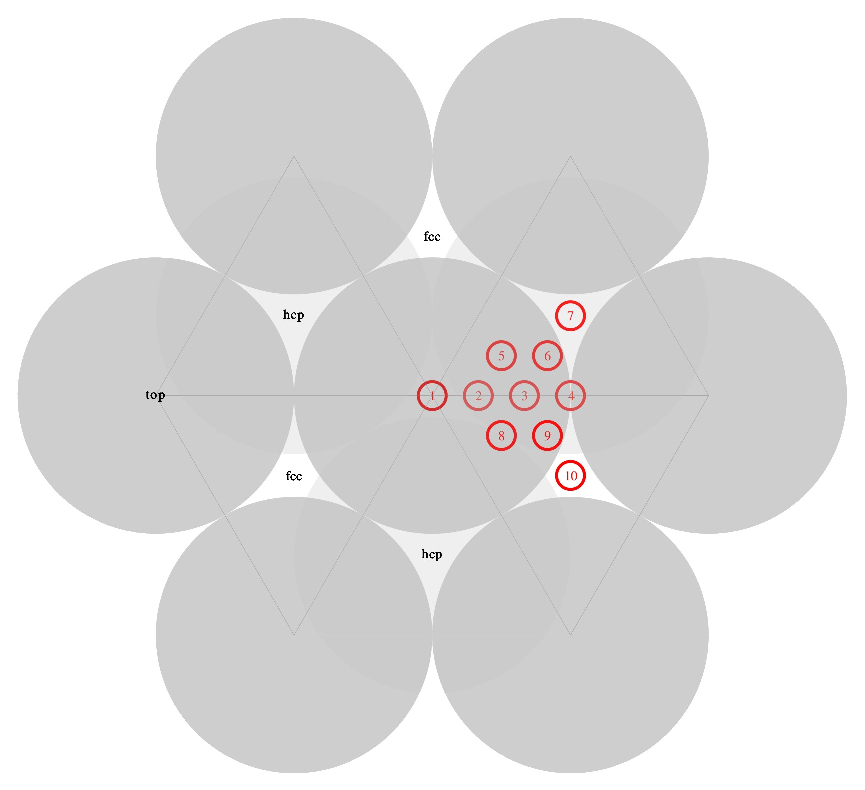
\includegraphics[width=0.7\textwidth]{SurfaceSites}
\caption{Ten Surface Sites for the PES.}
\label{surfacesites}
\end{figure}
The points 1 to 4 scan the region from the top site (1) to the bridge site (4). (1)-(5)-(7) maps out the straight line from the top site to the hcp-hollow site (7) and (1)-(8)-(10) from the top site to the fcc-hollow site (10). (6) and (9) sample the site of the metal atom. The H-atom should be moved perpendicular (that is, keeping the $x$- and $y$-coordinates fixed) to each of these sites starting from 6\,\AA~above the surface to the bottom layer of the slab in steps of 0.2\,\AA. The $x$- and $y$-coordinates of the points can be calculated as shown in Tab.\,\ref{calsusi}.
\begin{table}[h!]
\centering
\caption{How to calculate the $x$- and $y$-positions of the ten surface sites.}
\label{calsusi}
\begin{tabular}{ccc}
\hline\hline
Site&$x$-coordinate&$y$-coordinate\\
\hline
1&0.0						&0.0\\
2& $\frac{a_0}{6\sqrt{2}}$	&0.0\\
3& $\frac{a_0}{3\sqrt{2}}$	&0.0\\
4& $\frac{a_0}{\sqrt{8}}$	&0.0\\
5& $\frac{a_0}{4 \sqrt{2}}$	&$\frac{\sqrt{3}}{12\sqrt{2}}a_0$\\
6& $\frac{5}{12\sqrt{2}}a_0$&$\frac{\sqrt{3}}{12\sqrt{2}}a_0$\\
7& $\frac{a_0}{\sqrt{8}}$	&$\frac{\sqrt{3}}{6\sqrt{2}}a_0$\\
8& $\frac{a_0}{4\sqrt{2}}$	&$-\frac{\sqrt{3}}{12\sqrt{2}}a_0$\\
9& $\frac{5}{12\sqrt{2}}a_0$&$-\frac{\sqrt{3}}{12\sqrt{2}}a_0$\\
10&$\frac{a_0}{\sqrt{8}}$ 	&$-\frac{\sqrt{3}}{6\sqrt{2}}a_0$\\
\hline\hline
\end{tabular}
\end{table}\newline\noindent
Extract from the OUTCAR-files of each calculation the `energy sigma $\rightarrow$ 0' -energy. The energy when the H-atom is above the fcc-site and 6.0\,\AA~above the surface serves also as \textbf{reference energy}.
\subsection{The AIMD-trajectories}
Part of the fitting procedure also includes taking geometries at which the metal-atoms are not on their equilibrium positions and the H-atom is on other plausible positions that it might take up during a trajectory. To sample that configuration space, we take geometries from an AIMD-trajectory calculated for the very same system. Because we have not yet found out what kind of AIMD-geometries might give the best contribution to a fit, it is best to calculate roughly 20 AIMD-trajectories and use geometries from each of these trajectories as input for the fit.\\
I have no idea how to actually calculate AIMD trajectories, but I hope someone else can oblige here.

\section{Fitting the Potential Energy Surface with EMT}
\subsection{The parameters}
The Effective Medium Theory developed by N\o rskov \emph{et al.}\,\cite{jacobsen96,emt80,emt82,emt87} has seven parameters per species which are related to the physical properties of the species.\\
There are $\eta_2$, $n_0$, $E_0$, $\lambda$, $V_0$, $\kappa$ and $s_0$.
$s_0$ is the neutral sphere radius. It is calculated (Eq.\,) as follows from the lattice constant $a_0$ determined in the bulk-calculations:
\begin{equation}
s_0 = \frac{a_0}{\beta' \sqrt{2}}
\end{equation}
Here, $\beta'$ is a geometrical factor for the fcc-crystal:
\begin{equation}
\beta' = \frac{\sqrt[2]{16 \pi /3}}{\sqrt{2}}
\end{equation}
$E_0$ is the cohesive energy (sublimation energy) which can be found in literature. 
Together with $\lambda$, $E_0$ and $s_0$ are directly related to the bulk modulus:\\
\begin{equation}
B = -\frac{E_0 \lambda^2}{12 \pi s_0}
\end{equation}
$s_0$ is furthermore related to the shear modulus, together with $\kappa$, $\eta_2$ and $V_0$:\\
\begin{equation}
C_{44} = \frac{s\cdot V_0\cdot \kappa (\beta'\eta_2-\kappa)}{8\pi s_0}
\label{c44}
\end{equation}
We don't know how large $s$ is, yet, but it should be somewhere between 2 and 3.\\
$n_0$ is a parameter relating to the individual density of the species and responsible for the coupling between species.\\
\subsubsection*{Recommendations for the parameters}
\textbf{Parameters for the metal} (Me)\\
All the parameters apart for $E_{0,Me}$ should have positive values.
$s_{0,Me}$ and $E_{0,Me}$ should be kept constant during the fit to reproduce the most important bulk properties. If you would vary $s_{0,Me}$, you would also change the lattice constant of your metal and that does not make very much sense since you spent a lot of time actually finding the right one. Varying $E_{0,Me}$ will mostly destabilise the fit anyway, but it will also lead to PES which melt at very low temperatures (if $E_{0,Me}$ is too small) or not at all. So, it's not advisable to change this parameter. $\lambda_{Me}$ is a parameter you can keep fixed during the fitting procedure so the experimental bulk-modulus is reproduced. Actually fitting it might improve the fit slightly, but then, you won't reproduce the bulk-modulus as accurately anymore.\\
Furthermore, you should keep $\kappa_{Me}$, $\eta_{2,Me}$ and $V_{0,Me}$ such that they roughly reproduce the shear-modulus. For Au, $C_{44}$ (without $s$) should be $C_{44} \ge 10^{10}$ and best $C_{44} \ge 1.2 \cdot 10^{10}$. The melting temperature of the slab is in some obscure way related to $C_{44}$. I haven't figured out in which way, yet, but if your shear modulus gets too small (smaller than the numbers I recommend here), the surface will start disintegrating at unreasonably low temperatures.\\
As far as I've seen it, there aren't any issues related to $n_{0,Me}$..\\
\begin{table}[h!]
\centering
\caption{Recommendations for the metal parameters.}
\label{calsusi}
\begin{tabular}{ccc}
\hline\hline
Parameter&Relation to metal properties&Recommendation\\
\hline
$s_0$& $s_0= \frac{a_0}{\beta' \sqrt{2}}$& fix\\
$E_0$& Cohesive/Sublimation Energy& fix\\
$\lambda$&$B = -\frac{E_0 \lambda^2}{12 \pi s_0}$& (fix)\\
$\eta_2$, $\kappa$, $V_0$&$C_{44} = \frac{s\cdot V_0\cdot \kappa (\beta'\eta_2-\kappa)}{8\pi s_0}$& restrain\\
$n_0$& density& none\\
\hline\hline
\end{tabular}
\end{table}
\textbf{Parameters for Hydrogen}\\
There is no experimental data for metallic hydrogen that I know of. I therefore recommend to use the values suggested by Strömquist \emph{et al}\,\cite{strom98} as first guess but try to vary all of them during the calculations.\\
In general, you should not fit all hydrogen parameters at once, because that will destabilise the fit; if you are fitting $s_{0,H}$, $E_{0,H}$ should not fitted simultaneously and vice versa. The values suggested by Strömquist \emph{et al} for $s_{0,H}$ and $E_{0,H}$ result in good fits, so you do not necessarily need to fit them. If you decide to do so, for fitting $s_{0,H}$, I would recommend to set a guess-$s_{0,H}$ before you start the actual fitting. The estimated lattice constant for metallic hydrogen is around 0.88\,\AA~resulting in $s_{0,H}=0.49$\,\AA\,\cite{wigner35}, you should take note, though, that lowering $s_{0,H}$ also reduces the density the H-atom feel. In the nonadiabatic calculations, this would decrease the friction coefficient.\\
If you are fitting $s_{0,H}$ or $E_{0,H}$, I would first fit them with some of the other parameters and after that perform another fit in which you take the new values for $s_{0,H}$ or $E_{0,H}$ from your previous fit, but optimise the other parameters separately.\\
\begin{figure}[H!!!]
\begin{verbatim}
   eta2=             5.4254d0
     n0=             0.182205d0
     E0=            -2.37100000
 lambda=             7.72709d0
     V0=             0.427d0
  kappa=             8.86282d0
     s0=             0.68041100
\end{verbatim}
\caption{Exemplary file for the H-parameters. File contains the values suggested by Strömquist \emph{et al}. Please don't change the order of the parameters.}
\label{Mdtianfit}
\end{figure}
\subsection{Performing the fit}
\begin{figure}[H!!!]
\begin{verbatim}
projectile H 1.0079 7 'fitdata/emt573_H.nml' ver 0
lattice Au 196.96657 7 'fitdata/emt573_Au.nml' ver 0
pes emt
celldim 2 2 4 x
rep 1 1
conf fit au111_2x2x4.POSCAR 10 987
aimd 700 200 0.00
evasp -24.995689d0  ! A value for Au 2x2
fitconst 14 1 2 3 4 5 6 7 8 9 10 11 12 13 14
maxit 1
\end{verbatim}
\caption{Exemplary input-file for the fit in the MD\_tian Programm.}
\label{Mdtianfit}
\end{figure}
The input-file (cf Fig.\,\ref{Mdtianfit}) for the fit begins with the specification of the two species fitted. `projectile' classifies the projectile, in our case, the hydrogen atom. `lattice' specifies the metal slab. The flag is followed by the name of the projectile, its mass, the number of parameters, the file-name of the file that contains the starting parameters, the algorithm and the number of layers that should be kept fixed for eventual MD-simulations. The last two variables can be safely ignored for fitting. Next, `pes' declares for which theory the PES should be fitted. `celldim' records the dimensions of your input-cell as described for the optimisation of the H/Metal-system. `rep' organises how many times your cell should be replicated to produce a cell that is fit for EMT-usage. `rep 1 1' is a reasonable choice. 
`conf' determines if the program is going to be doing MD-simulations or fitting. For fitting, `conf' should be followed by `fit', the name of the POSCAR-file that contains your equilibrium structure with the H-atoms 6.0\,\AA~above the surface, the number of the AIMD-trajectory you would like to fit (in this case 10) and the number of the fit (in this case 987).\\
`aimd' controls the AIMD-contribution. The flag is followed by the number of Equilibrium-DFT-Points you would like to use, then by the number of AIMD-DFT-points and finally by de\_aimd\_max which determines how the AIMD-points should be chosen. If it is set to 0.0, then the points will be chosen in regular intervals from the trajectory. For larger values, a point is only then used in fitting if its energy-difference to the proceeding point is larger than de\_aimd\_max.\\
`evasp' controls the reference energy. It is followed by the energy a hydrogen atom has at 6.0\,\AA~above an equilibrated Au-surface (see previous section for determination of the reference energy).\\
`fitconst' determines which parameters should be kept fixed. Thus, the integer behind it is the number of fixed parameters in the fit, followed by the numbers corresponding to the fixed parameter. The numbers are assigned as follows (Tab.\,\ref{nopar}).\\
\begin{table}[h!]
\centering
\caption{Number of parameter for fitting.}
\label{nopar}
\begin{tabular}{rrrr}
\hline\hline
No.&Parameter&No.&Parameter\\
\hline
1&$\eta_{2,H}$	&8&$\eta_{0,metal}$\\
2&$n_{0,H}$		&9&$n_{0,metal}$\\
3&$E_{0,H}$		&10&$E_{0,metal}$\\
4&$\lambda_{H}$	&11&$\lambda_{metal}$\\
5&$\kappa_{H}$	&12&$\kappa_{metal}$\\
6&$V_{0,H}$		&13&$V_{0,metal}$\\
7&$s_{0,H}$		&14&$s_{0,metal}$\\
\hline\hline
\end{tabular}
\end{table}
`maxit' Maximal number of iteration. Followed by the maximal number of iterations. 100 is a good choice here.\\
\subsubsection*{Recommendations for the fitting}
Use a ratio of 5:2 between your Equilibrium- and AIMD-DFT Points. This appears to give good results. But we should do more detailed testing here.\\
Some AIMD-trajectories will work better for the fit than others. In my experience, trajectories in which the hydrogen atom spends a long time subsurface are not quite as suited as single- or double bounce trajectories. In our fitting procedure, you can decide between either taking regularly spaced points from the AIMD-trajectory (de\_aimd\_max = 0.0) or only such points that differ by a certain energy from the previous point (de\_aimd\_max = x). In my experience, taking equally spaced points works better. Also, you can decide points up to a certain energy should be taken into account (e\_max). In the program, this value is set to 20\,eV which I found to be suited best.
\subsection{After the Fit}
After the fit, the physically reasonable behaviour of the fit and its convergence needs to be determined. To check the convergence, calculate the rms to the input-data and the rms to the remaining AIMD-trajectories. If those values are both below 190\,meV, the fit can be considered a candidate.

\subsubsection*{Checking the Physical Behaviour of the Fit}
The first check is calculating $C_{44}$ (cf Eq.\,\ref{c44}). If the fit's $C_{44}\ll s\cdot1.2\cdot10^{10}$ the metal-surface will probably disintegrate at a too low temperature. You can test this by running MD-trajectories for different temperatures which propagate the motion for the metal-surface for several pico-seconds and by checking if the metal-slab still retains its shape as a surface after the trajectories.\\
Furthermore, you should also check if the H-atom can abstract metal-atoms from the surface. For that, you calculate the energy an H-atom has at 6\,\AA~above the surface. Then do the same calculations, only additionally to the H-atom at 6\,\AA, remove a metal-atom from the surface and place it at the distance of the H-metal-bond above the H-atom. With that I mean: Form a vacancy in the surface and use the atom from this vacancy to create a metal-H-molecule that is also 6\,\AA~above the surface.\\
Calculate from the difference the energy $\zeta$ that is need to form an H-metal molecule from a surface atom and an H-atom. We should probably implement a subroutine into the fitting procedure that does that automatically at the end of the fit.\\
\begin{equation}
\zeta = \Delta_\mathrm{f} H^\circ(\mathrm{Au_{s\rightarrow g}})-\Delta_\mathrm{f}H^\circ(\mathrm{Au-H})
\label{zeta}
\end{equation}
Compare the value to experimental values. $\zeta$ can be calculated by subtracting the metal-H-formation energy from the sublimation energy of the metal (cf Eq.\,\ref{zeta}). The value obtained for your fit should not be much below it.
\begin{table}[h!]
\centering
\caption{The arts of metal-H formation.}
\label{auh}
\begin{tabular}{ccccc}
\hline\hline
Metal&$\Delta_\mathrm{f} H^\circ(\mathrm{Au_{s\rightarrow g}})$(eV)&$\Delta_\mathrm{f}H^\circ(\mathrm{Au-H})$(eV)&bond length (\AA)&$\zeta$ (eV)\\
\hline
Au&3.8\cite{hildenbrand62}&2.99\,\cite{kant79}&1.52 (CRC)&0.8\\
Cu&&2.53\,\cite{kant79}&&\\
Ag&&2.19\,\cite{kant79}&&\\
Ni&&2.58\,\cite{kant79}&&\\
\hline\hline
\end{tabular}
\end{table}

\subsection{Possible issues}
If the fit has problems converging, you can first try fitting to the equilibrium-GGA-DFT-points and use the resulting parameters as input in a new fit where you then include both the equilibrium-DFT-points and the aimd-DFT-points.
Last but not least: form a circle of salt around your computer before starting the fitting and sacrifice a few drops of water to Thoth.\\


\bibliography{bib}% Produces the bibliography via BibTeX.
\end{document}